\subsection{Classificação de Cor}
Este é considerado o "Hello World" de SOMs. A maioria dos tutoriais publicados no
SOMs usam a classificação de cor SOM como seu principal exemplo. Isto é para uma muito
uma boa razão. Ao passar por este exemplo, o conceito de SOMs pode ser solidamente
apreendido. A razão pela qual a classificação de cor é bastante fácil de entender é por causa da
quantidade relativamente pequena de dados utilizados, bem como o aspecto visual dos
dados.

A classificação de cores do SOM usam apenas três pesos por mapa e nós de entrada.
Estes pesos representam a tripla (r, g, b) para a cor. Por exemplo, as cores podem
ser apresentado à rede, (1,0,0) para o vermelho (0,1,0) para o verde, etc A meta para
a rede aqui, é para aprender a representar todas essas cores de entrada em sua grade de duas dimensões,
mantendo as propriedades intrínsecas de tal como mantendo as
relações topológicas entre os vetores de entrada. Com isso em mente, se azul escuro
e azul claro são apresentados ao SOM, eles devem acabar ao lado do outro
da grelha de rede.

Para ilustrar o processo passo a passo através do algoritmo para a
aplicação de classificação da cor. O primeiro passo representa a inicialização da rede. A Figura \ref{fig:initial-node}
mostra uma rede recém inicializado. Cada quadrado representa um nó da rede.

\begin{figure}[ht]
\centering
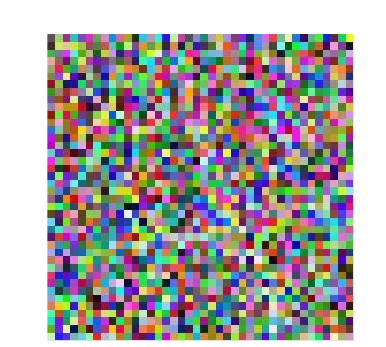
\includegraphics[width=0.7\textwidth]{imgs/initial-node.png}
\caption{Disposição inicial dos neurônios}
\label{fig:initial-node}
\end{figure}


O segundo passo é escolher um vetor de forma aleatória a partir dos vetores de entrada.
O passo 2 escolhe um vetor de forma aleatória a partir dos vectores de entrada. Oito vetores de entrada
são utilizados neste exemplo, que vão do vermelho para o amarelo para verde escuro. Em seguida,
o Passo 3 passa por cada nó e encontra BMU, conforme descrito anteriormente. A Figura \ref{fig:bmu-node}
mostra o BMU sendo selecionado na rede 4x4. A etapa 4 do
algoritmo calcula o raio vizinhança. Isto também é mostrado na Figura \ref{fig:bmu-node}. Todos
os nós em vermelho estão dentro do raio. No passo 5, em seguida, aplica-se o aprendizado
funções para todos estes nodos. Baseia-se na sua distância a partir do neurônio vencedor. O
neurônio vencedor (vermelho escuro) aprende mais, enquanto nós, na periferia do raio (luz
rosa) aprendem o mínimo. Nós fora do raio (branco) não aprendem nada.

\begin{figure}[ht]
\centering
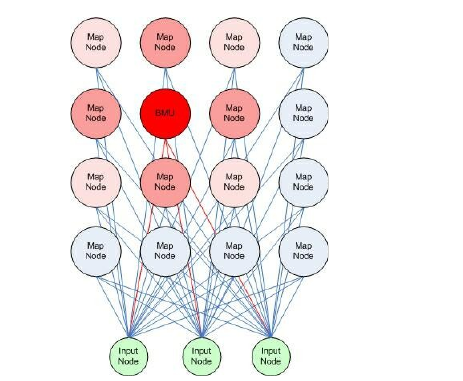
\includegraphics[width=0.7\textwidth]{imgs/node-bmu.png}
\caption{Nó vencedor}
\label{fig:bmu-node}
\end{figure}

Em seguida, volte para a Etapa 2 e repita. A Figura \ref{fig:final-node} mostra um SOM treinado,
representando todas as cores de oito entradas de cores. Observe como a luz verde fica ao lado do verde escuro,
e vermelho está ao lado de laranja.

\begin{figure}[ht]
\centering
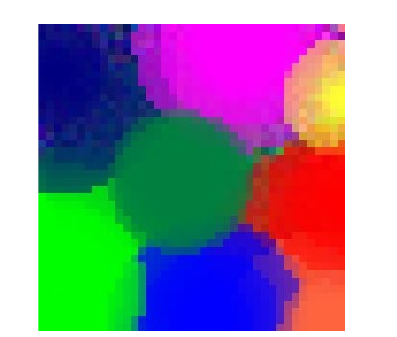
\includegraphics[width=0.5\textwidth]{imgs/final-node.png}
\caption{Estrutura do nó final}
\label{fig:final-node}
\end{figure}